\documentclass[sigconf, nonacm]{acmart}

\usepackage{booktabs}
\usepackage{amsmath}
\usepackage{pgfplots}
\usepackage[ruled,linesnumbered,noend]{algorithm2e}
\pgfplotsset{compat=1.17}
\usetikzlibrary{positioning,arrows.meta}

\settopmatter{printacmref=false, printccs=false, printfolios=true}
\renewcommand\footnotetextcopyrightpermission[1]{}
\setcopyright{none}

\newcommand{\sys}{OntoDB}
\newcommand{\code}[1]{\texttt{#1}}
\newtheorem{lemma}{Lemma}

\begin{document}

\title{Beyond the Sort Order: Hierarchy Intervals and Vector Indexes\\in a B+~Tree Ontology Store}

\author{Lam Nguyen}
\affiliation{%
  \institution{Microsoft}
  \country{USA}}
\email{lamng3.work@gmail.com}

\renewcommand{\shortauthors}{Nguyen}

\begin{abstract}
An ontology store is asked two kinds of question. \emph{Structural} ones, such as ``which instances have a type at or below class $C$'', have an exact answer in the data. \emph{Semantic} ones, such as ``which terms are closest in meaning to $t$'', have no answer in the data and need a similarity measure. Sorted indexes are the workhorse of triple stores, and it is tempting to think that sorted means close. We show it does not. A bandwidth argument proves that no linear order of points in two or more dimensions keeps all neighbors within a short scan, and on the Gene Ontology with sentence embeddings the best order we tried, the postorder of the class hierarchy, finds only 38\% of a term's ten nearest neighbors within 100 positions. We then use the order for what it can do. A postorder numbering of the class DAG with an interval set per class, kept in the engine's own B+~tree, turns ``everything under $C$'' into a few range scans. Against materializing the RDFS closure, it stores 8.1$\times$ fewer triples and a 4.2$\times$ smaller file on synthetic instances over the Gene Ontology, and answers within 1.8$\times$ of its page reads; against rewriting the query it reads 48$\times$ fewer pages for large classes. For similarity we add vector indexes inside the same engine: exact search, IVF with posting lists stored as B+~tree key ranges, product quantization, and HNSW. Pre-filtering through the intervals is exact and 10$^2$--10$^4\times$ faster than any index strategy for classes below about 1\,000 members; beyond 5\,000, a masked HNSW search wins. The filter is correlated with the vectors: for a query outside a small class, post-filtering IVF finds 7\% of the right answers, because the neighbors of a term tend to lie under the term's own ancestors, not under the class asked for. We implement everything in \sys, an open-source C++ ontology database, and every number in this paper regenerates from one script.
\end{abstract}

\maketitle

\section{Introduction}

Ontologies are stored and queried as graphs of triples, and the engines that hold them index those triples in sorted structures: B+~trees over permutations of subject, predicate, and object~\cite{rdfox}. A sorted index answers a bound prefix with one range scan, and this is the right tool for the questions it was built for. Two newer questions are not among them.

The first asks about the hierarchy. A query for the instances of \code{Material} should return the instances of \code{Metal} too, because \code{Metal} is a subclass. The second asks about meaning: given a term, which other terms are close to it? This is the question behind retrieval over ontologies, term matching, and ontology alignment, and it is what a vector index answers. The two questions meet in the third, ``the terms most similar to $t$ that lie under $C$''.

This paper asks what a B+~tree ontology store should do about them, and it makes four contributions.

\begin{enumerate}
\item \textbf{Order is not similarity.} We prove that any linear order of a $d$-dimensional point set separates some neighbors by $\Omega(n^{(d-1)/d}/d)$ positions (Lemma~\ref{lem:bw}), and measure how much locality the orders available to a store do give on a real ontology with real embeddings (Section~\ref{sec:order}). A hierarchy order is far better than first-seen ids and still leaves most neighbors out of a short scan.
\item \textbf{Hierarchies are intervals.} We label the class DAG so that the descendants of a class are a few integer intervals, bound the number of intervals by the number of non-tree edges (Lemma~\ref{lem:size}), and keep them in a B+~tree beside the triples. On the Gene Ontology the mean class needs 2.0 intervals; against materialization it saves 8.1$\times$ the triples, and against rewriting it saves 48$\times$ the page reads (Section~\ref{sec:labels}).
\item \textbf{Vector indexes in the engine.} We add exact, IVF, PQ, and HNSW search to the engine, and store IVF posting lists as key ranges of the same B+~tree that holds the triples (Section~\ref{sec:vectors}).
\item \textbf{Filtering by a class.} We compare pre-filtering, post-filtering, and masked search for ``nearest under $C$'', and show that in an ontology the filter is correlated with the vectors, which breaks the independence assumption behind the usual cost estimate (Section~\ref{sec:hybrid}).
\end{enumerate}

Everything is built in \sys{}, an open-source ontology database in C++20 (Section~\ref{sec:impl}); the benchmark is one script.

\section{Background and Related Work}

\paragraph{Triple stores and inference.} RDF stores keep triples in several sorted permutations; \sys{} keeps three (SPO, POS, OSP), enough to make every bound/unbound pattern a prefix scan. RDFS entailment is usually either \emph{rewritten} into the query or \emph{materialized} at write time, as RDFox does~\cite{rdfox}, with maintenance by counting or by delete-and-rederive~\cite{gupta1993}. Section~\ref{sec:labels} adds a third option that stores no entailed triple.

\paragraph{Labelling a hierarchy.} Agrawal, Borgida, and Jagadish~\cite{agrawal1989} store a compressed transitive closure by numbering a spanning forest in postorder and giving each node a set of intervals; Grust~\cite{grust2002} numbers XML trees in pre- and postorder so axes become regions of a plane. We use the former, on class DAGs, inside a B+~tree store, and measure it against the other two ways to answer a type query.

\paragraph{Vector search.} Approximate nearest neighbor search has three families that matter here: inverted files and product quantization~\cite{jegou2011}, proximity graphs, of which HNSW~\cite{malkov2020} is the standard, and disk-oriented graphs such as DiskANN~\cite{subramanya2019}. FAISS~\cite{johnson2021} packages the first two. Pan, Wang, and Li survey vector database systems and the hybrid queries (attribute plus vector) that are hard for them~\cite{pan2024}. ACORN~\cite{patel2024} makes HNSW traverse only the nodes that pass a predicate.

\paragraph{Graph and RDF systems with vectors.} Neo4j offers an HNSW vector index queried from Cypher~\cite{neo4jvec}; Amazon Neptune Analytics offers vector similarity over graph nodes~\cite{neptunevec}; Fluree provides inline similarity functions and HNSW indexes for RDF~\cite{fluree}; GraphDB has had similarity indexes queried from SPARQL since version 8~\cite{graphdbsim}. In the documentation we read, none turns the class hierarchy into range-scannable intervals, in the engine that holds the triples, to restrict a vector search.

\paragraph{Embeddings of hierarchies.} Euclidean embeddings of names are what we use; hyperbolic embeddings~\cite{nickel2017} represent hierarchies more faithfully and would change the vectors, not the indexes.

\paragraph{Adaptive radix trees.} The ART~\cite{leis2013} orders keys by byte, so its range scan is lexical; DuckDB persists it~\cite{duckdbart}. We discuss it in Section~\ref{sec:discussion}.

\section{System Overview}
\label{sec:overview}

\autoref{fig:arch} shows what \sys{} holds. The triples are dictionary-encoded and indexed in three B+~tree permutations, as before. The class hierarchy is read from the \code{rdfs:subClassOf} triples, labelled, and kept in a fourth B+~tree. Vectors, one per term id, sit in a store beside them, with three optional indexes; the IVF index is again a B+~tree. A hybrid query touches the label tree and one vector index, never the triple trees.

\begin{figure}[t]
\centering
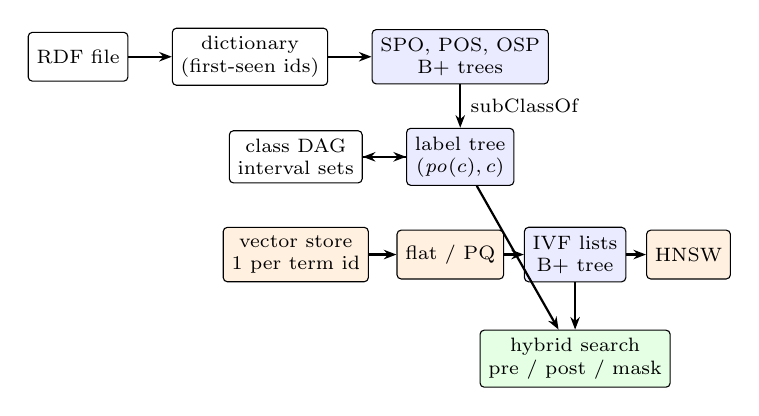
\begin{tikzpicture}[font=\scriptsize,node distance=0.35cm and 0.35cm,
  box/.style={draw,rounded corners=1.5pt,minimum height=0.62cm,inner sep=3pt,align=center,fill=white},
  tree/.style={box,fill=blue!8},
  vec/.style={box,fill=orange!12},
  arr/.style={-{Stealth[length=1.6mm]},thick}]
\node[box] (rdf) {RDF file};
\node[box,right=0.55cm of rdf] (dict) {dictionary\\(first-seen ids)};
\node[tree,right=0.55cm of dict] (spo) {SPO, POS, OSP\\B+ trees};
\node[tree,below=0.55cm of spo] (lab) {label tree\\$(\mathit{po}(c),c)$};
\node[box,left=0.55cm of lab] (hier) {class DAG\\interval sets};
\node[vec,below=0.55cm of hier] (vs) {vector store\\1 per term id};
\node[vec,right=0.35cm of vs] (flat) {flat / PQ};
\node[tree,right=0.25cm of flat] (ivf) {IVF lists\\B+ tree};
\node[vec,right=0.25cm of ivf] (hnsw) {HNSW};
\node[box,fill=green!10,below=0.6cm of ivf] (hy) {hybrid search\\pre / post / mask};
\draw[arr] (rdf) -- (dict);
\draw[arr] (dict) -- (spo);
\draw[arr] (spo) -- node[right]{\scriptsize subClassOf} (lab);
\draw[arr] (lab) -- (hier) node[midway,above]{\scriptsize };
\draw[arr] (hier) -- (lab);
\draw[arr] (vs) -- (flat);
\draw[arr] (flat) -- (ivf);
\draw[arr] (ivf) -- (hnsw);
\draw[arr] (lab) -- (hy);
\draw[arr] (ivf) -- (hy);
\end{tikzpicture}
\caption{What \sys{} holds. Blue boxes are B+~trees of the same kind; the class DAG is rebuilt from the \code{subClassOf} triples, and vectors come from an external embedding model.}
\label{fig:arch}
\end{figure}

\section{What a Sorted Index Can Say About Meaning}
\label{sec:order}

\paragraph{The order of \sys's trees.} A triple is a 24-byte key of three dictionary ids compared with \code{memcmp}. The dictionary assigns ids densely, in first-seen order, and the loader interns the terms of each statement in file order. So the order of every tree is the order in which terms first appeared in the input. Two classes are adjacent in the index only if they were adjacent in the file.

\paragraph{No order holds similarity.}

\begin{lemma}[Bandwidth]\label{lem:bw}
Let $G$ have $n$ vertices and diameter $D$. In every linear order of the vertices some edge joins vertices at least $(n-1)/D$ positions apart.
\end{lemma}
\begin{proof}
The first and last vertices of the order are $n-1$ apart and joined by a path of at most $D$ edges; some edge of the path covers at least $(n-1)/D$.
\end{proof}

For the neighbor graph of a $d$-dimensional grid with $n=k^d$ points (diameter $d(k-1)$) this gives $(k^d-1)/(d(k-1)) \ge k^{d-1}/d$ positions, in any order. A scan of width $w$ cannot contain all neighbors unless $w$ is that large. Space-filling curves keep neighbors close on average and need several scans to cover a query ball; they do not escape the lemma.

\paragraph{How much locality do real orders give?} We took the Gene Ontology (release 2026-07-26, without obsolete terms: 38\,092 classes, 57\,456 \code{is\_a} edges), embedded each term's name with \code{all-MiniLM-L6-v2}~\cite{reimers2019} (384 dimensions, on a CPU, 45 s), and for 2\,000 random terms took the ten nearest by cosine. For each order of the terms, \autoref{tab:order} gives the share of those neighbors within $\pm W$ positions.

\begin{table}[t]
\caption{Share of the 10 nearest neighbors (by cosine) found within $\pm W$ positions of a term, and the median position gap to the nearest neighbor. GO, 38\,092 terms, 2\,000 queries.}
\label{tab:order}
\small
\begin{tabular}{@{}lrrrrrr@{}}
\toprule
Order & gap & $\pm$50 & $\pm$100 & $\pm$500 & $\pm$1000 & $\pm$5000 \\
\midrule
dictionary id (first seen) & 1739 & .195 & .211 & .258 & .284 & .438 \\
hierarchy, deepest parent & 45 & .328 & .377 & .498 & .561 & .735 \\
hierarchy, first parent & 37 & .319 & .366 & .481 & .546 & .726 \\
label, alphabetical & 1749 & .310 & .334 & .379 & .408 & .558 \\
random & 10823 & .003 & .005 & .024 & .049 & .242 \\
\bottomrule
\end{tabular}
\end{table}

\begin{figure}[t]
\centering
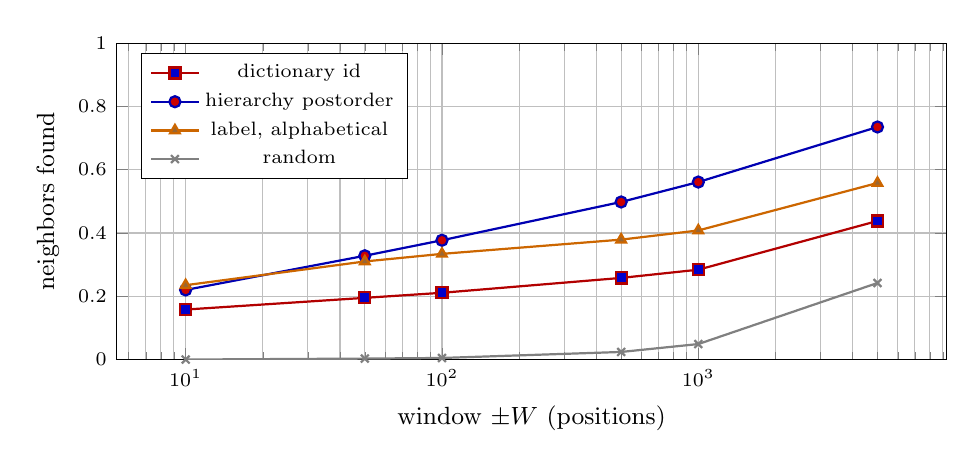
\begin{tikzpicture}
\begin{axis}[width=\columnwidth,height=5.6cm,xmode=log,xlabel={window $\pm W$ (positions)},ylabel={neighbors found},ymin=0,ymax=1,grid=both,legend pos=north west,legend style={font=\scriptsize},tick label style={font=\scriptsize},label style={font=\small}]
\addplot+[mark=square*,color=red!70!black,thick] coordinates {(10,0.158) (50,0.195) (100,0.211) (500,0.258) (1000,0.284) (5000,0.438)};
\addlegendentry{dictionary id}
\addplot+[mark=*,color=blue!70!black,thick] coordinates {(10,0.22) (50,0.328) (100,0.377) (500,0.498) (1000,0.561) (5000,0.735)};
\addlegendentry{hierarchy postorder}
\addplot+[mark=triangle*,color=orange!80!black,thick] coordinates {(10,0.235) (50,0.31) (100,0.334) (500,0.379) (1000,0.408) (5000,0.558)};
\addlegendentry{label, alphabetical}
\addplot+[mark=x,color=gray,thick] coordinates {(10,0) (50,0.003) (100,0.005) (500,0.024) (1000,0.049) (5000,0.242)};
\addlegendentry{random}
\end{axis}
\end{tikzpicture}

\caption{The data of \autoref{tab:order}: neighbors found in a window of $\pm W$ positions, by order.}
\label{fig:order}
\end{figure}

Three things follow. First, the hierarchy's postorder is the best order, and it is much better than \sys's first-seen ids: the nearest neighbor is 45 positions away instead of 1\,739. Second, even so, a scan of 100 positions finds 38\% of the ten neighbors, and a window of $\pm$1000 positions (2.6\% of the ontology) still misses 44\%; Lemma~\ref{lem:bw} is not an artifact of the grid. Third, first-seen ids are not random: the Gene Ontology's ids were minted in related batches, so ids carry some locality (0.21 at $\pm$100) that depends on the file and not on the engine. Of the ten neighbors, 12\% are a parent or child and 32\% are within two \code{is\_a} steps; a two-step neighborhood holds 45 terms (0.12\% of the ontology), so hierarchy proximity is highly informative about meaning without being sufficient.

The order is therefore useful for structure and not a substitute for a vector index.

\section{Hierarchies as Intervals}
\label{sec:labels}

\paragraph{Labelling.} Let the class hierarchy be a DAG, after collapsing each cycle ($A \sqsubseteq B \sqsubseteq A$) into one class, since such classes are equivalent. Choose a spanning forest by taking, for each class with several parents, the parent with the longest path from a root. Number the forest's nodes $1..n$ in postorder, and let $\mathit{lo}(c)$ be the smallest number in the tree subtree of $c$. For a forest, $d$ is at or below $c$ iff $\mathit{lo}(c)\le \mathit{po}(d)\le \mathit{po}(c)$. For a DAG each class carries a \emph{set} of intervals, built bottom-up (Algorithm~\ref{alg:label}).

\begin{algorithm}[t]
\caption{Interval sets for a class DAG}\label{alg:label}
\small
\KwIn{edges $(c,p)$: $c$ is a subclass of $p$}
\KwOut{$\mathit{po}(c)$ and an interval set $I(c)$ for each class}
collapse strongly connected components (Tarjan), number them parents first\;
\For{each component $c$, parents first}{
  $\mathit{depth}(c) \gets 1 + \max_{p}\ \mathit{depth}(p)$ \tcp*{0 for a root}
  $\mathit{tp}(c) \gets$ the parent with the largest depth\;
}
number the forest $\{(c,\mathit{tp}(c))\}$ in postorder; record $\mathit{lo}(c)$\;
\For{each component $c$, children first}{
  $I(c) \gets \textsc{Merge}\big(\{[\mathit{lo}(c),\mathit{po}(c)]\} \cup \bigcup_{c\to v} I(v)\big)$ \tcp*{sort, join overlapping or adjacent}
}
\end{algorithm}

\begin{lemma}[Correctness]
$d$ is at or below $c$ iff $\mathit{po}(d)$ lies in an interval of $I(c)$.
\end{lemma}
\begin{proof}
Induction over the order in which Algorithm~\ref{alg:label} builds $I$: the numbers covered by $I(c)$ are exactly those of the descendants of $c$.
\end{proof}

\begin{lemma}[Size]\label{lem:size}
Let $E'(c)$ be the non-tree edges with tail at or below $c$. Then $|I(c)|\le 1+|E'(c)|$.
\end{lemma}
\begin{proof}
A descendant $d$ is reached from $c$ by a path. If it uses no non-tree edge, $d$ is in the tree subtree of $c$; otherwise let $v$ be the head of the last non-tree edge on it, and $d$ is in the tree subtree of $v$. So the covered set is $\mathrm{own}(c)\cup\bigcup_{e\in E'(c)}\mathrm{own}(\mathrm{head}(e))$, a union of $1+|E'(c)|$ intervals.
\end{proof}

The labelling takes $O(n+m)$ plus the merges. A tree needs one interval per class. We check Lemma~\ref{lem:size} on every class of the Gene Ontology and on 60 random DAGs in the test suite.

\paragraph{Index.} The labels go into B+~trees of \sys: key $(\mathit{po}(c),c,0)$ for the classes, and $(\mathit{po}(t),x,0)$ for each triple $(x,\mathit{type},t)$. The descendants of $c$, or the instances of $c$ and its subclasses, are one range scan per interval of $c$. An instance insert adds one key. Labels are rebuilt when the hierarchy changes (here in 15~ms for GO); incremental maintenance with gaps~\cite{agrawal1989} is not built. Dictionary ids are untouched: ids appear in three permutations, the log, and snapshots, and renumbering them to follow the hierarchy would rewrite all of it.

\subsection{Evaluation}

\paragraph{Setup.} Gene Ontology as above; LUBM(1)~\cite{lubm} with its ontology (43 classes, 103\,410 triples); and 200\,000 synthetic entities, one to three types each drawn uniformly from GO's classes (495\,552 triples), because GO has no instances. Release build on an Apple M2 Pro, one thread. Page reads are counted on a cold 64-frame buffer pool, the methodology of \sys's indexing benchmark.

\paragraph{Label size.} \autoref{tab:labels} shows that GO needs 76\,570 intervals for 38\,092 classes, 2.01 per class, 598 KiB in all; the closure it replaces has 393\,448 ancestor pairs, 9 MiB at 24 bytes each and one permutation. The spanning-forest rule matters little (deepest parent saves 13\%). The tail is long: one class has 741 intervals, bounded by Lemma~\ref{lem:size}. Labels build in 15 ms. Asking whether $d$ is below $c$ takes 27 ns against 775 ns for a search up the parents.

\begin{table}[t]
\caption{Interval labels for the Gene Ontology.}
\label{tab:labels}
\small
\begin{tabular}{@{}lrrrr@{}}
\toprule
Spanning-forest rule & non-tree edges & intervals & mean / p99 / max & build \\
\midrule
deepest parent & 19\,367 & 76\,570 & 2.01 / 17 / 741 & 14.9 ms \\
first parent & 19\,367 & 87\,769 & 2.30 / 22 / 740 & 14.4 ms \\
\bottomrule
\end{tabular}
\end{table}

\paragraph{Descendants of a class.} \autoref{tab:desc} compares the $B^+$-tree interval scans with a breadth-first search that scans POS once per class. For a class with a thousand or more descendants the intervals need 101 scans instead of 3\,304, 40 page reads instead of 694, and 0.5 ms instead of 9 ms.

\begin{table}[t]
\caption{Descendants of a class in GO, cold 64-frame pool, mean over up to 40 classes per row.}
\label{tab:desc}
\small
\begin{tabular}{@{}lrrrr@{}}
\toprule
Below $C$ & method & scans & page reads & $\mu$s \\
\midrule
10--99 & intervals & 5.9 & 5.8 & 59 \\
 & one scan per class & 30.6 & 16.3 & 149 \\
100--999 & intervals & 29.1 & 13.2 & 147 \\
 & one scan per class & 268.2 & 65.7 & 803 \\
1000+ & intervals & 101.3 & 40.1 & 528 \\
 & one scan per class & 3303.6 & 694.1 & 8998 \\
\bottomrule
\end{tabular}
\end{table}

\paragraph{Instances of a class.} \autoref{tab:types} compares the three strategies on the synthetic instances. Materializing the closure turns 495\,552 triples into 4\,017\,973 (8.1$\times$), the file from 63.6 to 309.5~MiB, and the load from 5.1 s to 180 s. The interval index adds 9.3 MiB (15\%) and 0.17 s. On queries, the interval index is close to the materialized store and far from rewriting: for a class with a thousand or more descendants it reads 265 pages against 182 (materialized) and 12\,803 (rewrite), and runs in 4.6 ms against 3.8 and 82 ms. All three return identical answers on every sampled class. On LUBM(1) the hierarchy is shallow (43 classes) and the three are within a factor of about two on every query; materialization adds 15\% to the triples. The benefit of intervals grows with the depth and breadth of the hierarchy, and LUBM has little of either.

\begin{table}[t]
\caption{Instances of $C$ on 200\,000 synthetic entities over GO, mean over 30 classes per row (cold 64-frame pool). Top: cost of the store.}
\label{tab:types}
\small
\begin{tabular}{@{}lrrr@{}}
\toprule
Strategy & triples & file (MiB) & load (s) \\
\midrule
rewrite & 495\,552 & 63.6 & 5.09 \\
intervals & 495\,552 & 72.9 & 5.26 \\
materialize & 4\,017\,973 & 309.5 & 180.31 \\
\bottomrule
\end{tabular}

\medskip
\begin{tabular}{@{}lrrrr@{}}
\toprule
Below $C$ & strategy & answers & page reads & $\mu$s \\
\midrule
10--99 & intervals & 278 & 8.4 & 90 \\
 & rewrite & 278 & 87.5 & 571 \\
 & materialized & 278 & 6.6 & 444 \\
100--999 & intervals & 2\,954 & 40.9 & 1\,461 \\
 & rewrite & 2\,954 & 1\,153 & 7\,280 \\
 & materialized & 2\,954 & 22.5 & 987 \\
1000+ & intervals & 29\,904 & 264.8 & 4\,555 \\
 & rewrite & 29\,904 & 12\,803 & 82\,441 \\
 & materialized & 29\,904 & 182.0 & 3\,776 \\
\bottomrule
\end{tabular}
\end{table}

\section{Vector Indexes in the Engine}
\label{sec:vectors}

The engine keeps one unit-length float vector per term id, in memory, loaded from a checksummed file whose records name terms by spelling, so a file survives a dictionary that numbers terms differently. Embeddings come from outside; \sys{} stores and searches them. Four index families are available, each a different trade between exactness, memory, and build time.

\paragraph{Flat.} Score every vector: $O(nd)$ and exact. With 8-bit scalar quantization (one scale per vector, $s=\max|x|/127$) each coordinate is off by at most $s/2$, so for a unit query a score is off by at most $(s/2)\sqrt d$, in a quarter of the memory.

\paragraph{IVF.} Spherical $k$-means with $k$-means++ seeding~\cite{arthur2007} gives $L$ centroids; each vector goes to its nearest. A query scores the centroids and reads the $p$ nearest lists. The cost is $Ld + p(n/L)d$, minimal at $L=\sqrt{pn}$. The design choice is where the lists live: \emph{as key ranges of the B+~tree that holds the triples}. The pair $(\mathrm{list},\mathrm{row})$ is a key $(\mathrm{list},\mathrm{row},0)$, so a list is a prefix scan, an insert is a tree insert, and the lists page, cache, and latch like every other index of the engine. Under a filter the search keeps probing the nearest remaining lists until it holds $k$ allowed rows, so a filter that excludes everything near the query costs more instead of returning nothing.

\paragraph{Product quantization.} Cut a vector into $m$ pieces and replace each by the index of its nearest of 256 learned centers~\cite{jegou2011}: $m$ bytes per vector. A query builds $m$ tables of 256 dot products and scores a code as the sum of $m$ lookups, which equals the dot product with the decoded vector, so all the error is on the stored side.

\paragraph{HNSW.} The layered proximity graph of Malkov and Yashunin~\cite{malkov2020}, with the paper's neighbor-selection heuristic: a candidate is kept only if it is nearer the new node than to every neighbor already kept. Layer~0 allows $2M$ links. Search takes an optional filter and still crosses nodes it may not return.

\subsection{Evaluation}

38\,092 GO terms, 384 dimensions, 1\,000 query terms (the term itself excluded from its answer), exact search as ground truth, single thread. \autoref{tab:knn} gives selected points and \autoref{fig:knn} the recall--latency curves.

\begin{table}[t]
\caption{Vector indexes on GO (recall@10, mean time per query, memory of the structure, build time).}
\label{tab:knn}
\small
\begin{tabular}{@{}llrrrr@{}}
\toprule
Index & setting & recall & $\mu$s & MiB & build (s) \\
\midrule
flat float32 & exact & 1.000 & 2\,238 & 55.8 & --- \\
flat 8-bit & exact over codes & 0.996 & 4\,554 & 14.1 & --- \\
flat PQ $m{=}48$ & codes only & 0.778 & 819 & 1.7 & 10.4 \\
flat PQ $m{=}48$ & re-rank 100 & 0.998 & 905 & 1.7$^\dagger$ & 10.4 \\
IVF $L{=}512$ & nprobe 8 & 0.892 & 149 & 56.5 & 17.5 \\
IVF $L{=}512$ & nprobe 16 & 0.929 & 255 & 56.5 & 17.5 \\
IVF $L{=}512$ & nprobe 64 & 0.976 & 928 & 56.5 & 17.5 \\
IVF $L{=}512$, 8-bit & nprobe 16 & 0.926 & 263 & 14.8 & 17.5 \\
IVF $L{=}512$, PQ 96 & nprobe 16 & 0.839 & 178 & 4.2 & 38.4 \\
HNSW $M{=}16$ & $ef$ 10 & 0.993 & 44 & 59.7 & 15.0 \\
HNSW $M{=}16$ & $ef$ 40 & 0.997 & 108 & 59.7 & 15.0 \\
HNSW $M{=}32$ & $ef$ 160 & 0.999 & 474 & 63.4 & 28.0 \\
\bottomrule
\end{tabular}

\smallskip
{\footnotesize $^\dagger$ re-ranking reads the float vectors as well.}
\end{table}

\begin{figure}[t]
\centering
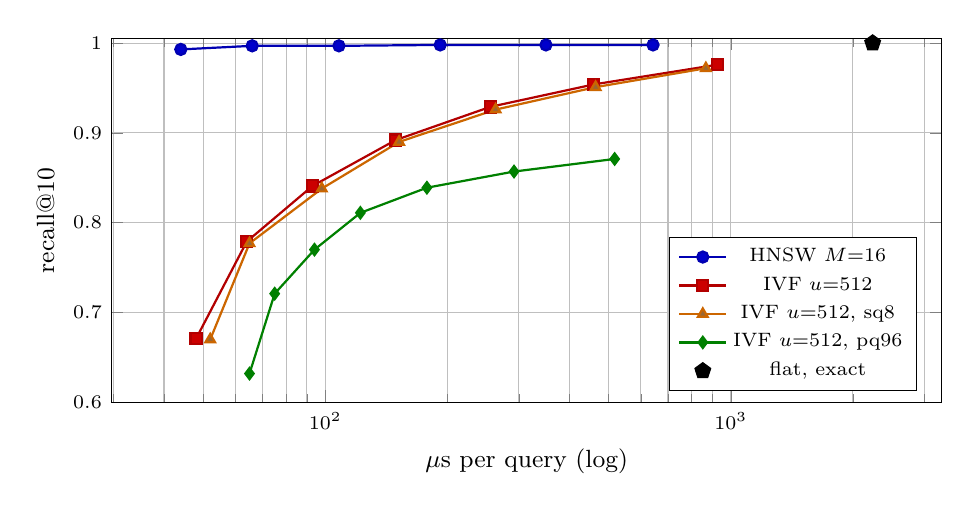
\begin{tikzpicture}
\begin{axis}[width=\columnwidth,height=6.2cm,xmode=log,xlabel={$\mu$s per query (log)},ylabel={recall@10},ymin=0.6,ymax=1.005,grid=both,legend pos=south east,legend style={font=\scriptsize},tick label style={font=\scriptsize},label style={font=\small}]
\addplot+[mark=*,color=blue!70!black,thick] coordinates {(44,0.993) (66,0.997) (108,0.997) (192,0.998) (350,0.998) (643,0.998)};
\addlegendentry{HNSW $M{=}16$}
\addplot+[mark=square*,color=red!70!black,thick] coordinates {(48,0.671) (64,0.779) (93,0.841) (149,0.892) (255,0.929) (459,0.954) (928,0.976)};
\addlegendentry{IVF $
u{=}512$}
\addplot+[mark=triangle*,color=orange!80!black,thick] coordinates {(52,0.67) (65,0.777) (98,0.838) (152,0.89) (263,0.926) (464,0.951) (868,0.972)};
\addlegendentry{IVF $
u{=}512$, sq8}
\addplot+[mark=diamond*,color=green!50!black,thick] coordinates {(65,0.632) (75,0.721) (94,0.77) (122,0.811) (178,0.839) (292,0.857) (517,0.871)};
\addlegendentry{IVF $
u{=}512$, pq96}
\addplot[only marks,mark=pentagon*,mark size=3pt,color=black] coordinates {(2238,1)};
\addlegendentry{flat, exact}
\end{axis}
\end{tikzpicture}

\caption{Recall@10 against time per query on GO (38\,092 vectors, 384 dimensions).}
\label{fig:knn}
\end{figure}

\paragraph{A baseline that is not slow by accident.} Our first run scored with a plain dot-product loop. A compiler may not vectorize it without \code{-ffast-math}, and the exact scan took 8.3~ms, which would have made the speed-ups look about twice as large: HNSW at $ef{=}10$ is 103 times faster than that baseline and 51 times faster than the vectorized one. With eight independent accumulators the exact scan takes 2.2~ms (13 Gflop/s), and every number here and in Section~\ref{sec:hybrid} uses that. We report it because a speed-up over ``exact'' depends entirely on how fast exact is.

\paragraph{What the numbers say.} HNSW dominates on this data: recall 0.993 at 44~$\mu$s, 51$\times$ faster than the exact scan, for 3.9~MiB of links on top of the vectors. IVF needs 255~$\mu$s for 0.929 and 928~$\mu$s for 0.976. IVF over the B+~tree is about 2.7$\times$ more expensive per scored row than a contiguous scan (about 157~ns against 59~ns): each entry is a decoded 24-byte key and a random read of the vector. That is the price of lists that page, cache, and update with the triples. The cost model holds in shape: more lists make a query cheaper until the centroid scan dominates ($L{=}2048$ pays 124~$\mu$s at nprobe~1). Product quantization is for memory, not speed, at this size: codes alone reach 0.78 or 0.88 recall in 1.7 or 3.5~MiB, and re-ranking the best 100 exactly recovers 0.998 and 1.000 but needs the float vectors. 8-bit codes keep 0.996 recall in a quarter of the memory and are slower than float32, because converting bytes to floats costs more than the cache misses they avoid at 56~MiB.

\paragraph{Caveat.} The queries are terms of the ontology, whose neighbors are also terms of it. Queries from outside the vocabulary, such as free text, would be harder, and we do not measure them.


\section{Filtering a Vector Search by a Class}
\label{sec:hybrid}

A hybrid query asks for the $k$ terms nearest $t$ that lie at or under class $C$. Let $s=|\mathrm{subtree}(C)|/n$. We compare four ways of answering it, all returning terms of the subtree only.

\begin{description}
\item[Pre-filter.] Resolve $C$ to its members first (one range scan per interval), then score only those, exactly. About $s\,n\,d$ work.
\item[Post-filter.] Ask the index for $k'>k$, keep the results under $C$ (a membership test is a binary search over $C$'s intervals; nothing is scanned), and multiply $k'$ by four until $k$ remain or the index is exhausted. If the filter were independent of the similarity, about $k/s$ candidates would be needed.
\item[Masked search.] Give the index a predicate, ``the row's label lies in an interval of $C$'', so a list scan or a graph walk skips rows outside $C$. Nothing is resolved in advance: each row the search touches costs one binary search. HNSW still crosses rows it may not return, to keep the graph connected, in the spirit of ACORN~\cite{patel2024}; IVF keeps probing lists until it has $k$ allowed rows.
\item[Auto.] Pre-filter when $C$ has at most 4\,096 classes, otherwise masked HNSW.
\end{description}

\paragraph{The filter is correlated with the vectors.} In an ontology the names of a class's descendants are close to the class and to each other, so the neighbors of a term tend to lie under the term's own ancestors. Of the unfiltered top 100 neighbors of a query from \emph{inside} $C$, 4\% to 72\% lie under $C$, rising with the size of $C$; for a query from \emph{outside} $C$ the share is 0\% to 12\%. The independence estimate $k/s$ is therefore wrong in both directions: post-filtering is cheap for an inside query and does not terminate usefully for an outside one.

\subsection{Evaluation}

For 20 classes in each of five subtree-size buckets we ran the ten nearest terms under $C$ for a query that is a member of $C$ (``inside'') and one that is not (``outside''), against the exact answer over the members. IVF uses 512 lists and 16 probes, HNSW $M{=}16$, $ef{=}64$. \autoref{tab:hybrid} gives recall and time.

\begin{table*}[t]
\caption{Ten nearest terms under a class $C$, by subtree size, query inside or outside $C$: recall@10 / $\mu$s per query. GO, 38\,092 terms. Masked and post-filtered searches use the index; pre-filter resolves the members and scores them exactly.}
\label{tab:hybrid}
\small
\begin{tabular}{@{}lccccc@{}}
\toprule
Strategy & $\le$10 & 11--100 & 101--1000 & 1001--5000 & $>$5000 \\
\midrule
\multicolumn{6}{@{}l}{\emph{query inside $C$}} \\
pre-filter & 1.00 / 3 & 1.00 / 9 & 1.00 / 62 & 1.00 / 292 & 1.00 / 1\,404 \\
post-filter, HNSW & 1.00 / 37\,553 & 1.00 / 1\,739 & 1.00 / 427 & 1.00 / 70 & 1.00 / 68 \\
post-filter, IVF & 0.86 / 903 & 0.87 / 558 & 0.93 / 293 & 0.98 / 198 & 0.99 / 211 \\
masked HNSW & 1.00 / 16\,653 & 1.00 / 15\,846 & 1.00 / 1\,150 & 1.00 / 183 & 1.00 / 105 \\
masked IVF & 1.00 / 1\,253 & 0.95 / 111 & 0.96 / 104 & 0.98 / 124 & 0.99 / 161 \\
auto & 1.00 / 3 & 1.00 / 9 & 1.00 / 59 & 1.00 / 269 & 1.00 / 95 \\
\midrule
\multicolumn{6}{@{}l}{\emph{query outside $C$}} \\
pre-filter & 1.00 / 3 & 1.00 / 9 & 1.00 / 62 & 1.00 / 291 & 1.00 / 1\,394 \\
post-filter, HNSW & 1.00 / 36\,654 & 1.00 / 27\,669 & 0.99 / 13\,607 & 1.00 / 5\,513 & 1.00 / 836 \\
post-filter, IVF & 0.07 / 966 & 0.02 / 1\,009 & 0.17 / 902 & 0.33 / 811 & 0.64 / 591 \\
masked HNSW & 1.00 / 16\,802 & 1.00 / 16\,611 & 1.00 / 8\,697 & 1.00 / 4\,424 & 1.00 / 900 \\
masked IVF & 1.00 / 1\,255 & 0.79 / 698 & 0.45 / 286 & 0.37 / 147 & 0.66 / 107 \\
auto & 1.00 / 3 & 1.00 / 9 & 1.00 / 62 & 1.00 / 295 & 1.00 / 860 \\
\bottomrule
\end{tabular}
\end{table*}

\paragraph{Exact pre-filtering wins for small classes.} Up to about 1\,000 members, resolving the members through the interval index and scoring them exactly takes 3 to 62~$\mu$s and is the exact answer. Every index-based strategy is slower, from 1.7$\times$ (masked IVF at 101--1\,000 members, at recall 0.96) to over 10\,000$\times$ (post-filtered HNSW on the smallest classes), because few of the vectors an index touches belong to the class. A graph search for a rare filter crosses most of the graph: masked HNSW reads 16~ms for a class of at most 100 members, the failure ACORN is designed to remove.

\paragraph{Post-filtering fails for outside queries.} IVF post-filter recall falls to 0.07 on the smallest classes and 0.64 on the largest; HNSW reaches full recall only by searching again and again (37~ms for a class of at most ten members, in six rounds).

\paragraph{Masked HNSW wins for large classes.} Above 5\,000 members it takes 105~$\mu$s inside and 900~$\mu$s outside, exact, against 1.4~ms for resolving and scoring the members.

\paragraph{Do not resolve the filter.} Our first masked search resolved $C$ by interval scans and built a bitmap per query. For a class of over 5\,000 members that took 669~$\mu$s, of which about 560~$\mu$s was resolving. Testing the label of each row the search touches, one binary search over a handful of intervals, brought the same search to 105~$\mu$s. This is where interval labels earn their keep a second time: they make membership an $O(\log|I(C)|)$ test with no scan.

\paragraph{A cost model for the crossover.} Let $c_m$ be the cost of pre-filtering per member (an interval scan, a hash lookup from term to row, and one dot product): from \autoref{tab:hybrid}, $c_m\approx 0.13$--$0.20~\mu$s for classes of a few hundred members or more. Pre-filtering beats a masked graph search when $|C|<T=c_h/c_m$, where $c_h$ is the masked search's time. For a query inside $C$, $c_h\approx 105$--$183~\mu$s, so $T\approx 800$--$1\,000$, which matches the observed crossing between the 101--1\,000 and 1\,001--5\,000 columns. For a query outside $C$ the masked walk costs 0.9--4.4~ms on classes of 1\,000 or more members, so $T$ is 7\,000--25\,000. A single threshold has to sit between the two; 4\,096 stays below the outside-query crossing and loses at most a factor of 3.8 at the inside-query one.

\paragraph{The auto rule.} With a threshold of 4\,096 members, auto matches the fastest strategy in every cell but one and is never slower than 0.9~ms. The exception is a class of 1\,001--5\,000 members with an inside query: 269~$\mu$s, against 70~$\mu$s for post-filtered HNSW and 183~$\mu$s for masked HNSW. Post-filtering would cost 5.5~ms for an outside query on the same class, so the rule gives up a factor of 3.8 in one cell to avoid a factor of 79 in its neighbor.


\section{Implementation}
\label{sec:impl}

\sys{} is a C++20 ontology database: a SPARQL subset over three B+~tree permutations of dictionary-encoded triples, with a buffer pool, a cost-based optimizer, strict two-phase locking, and ARIES recovery, checked by a crash harness. The semantic extension adds about 2\,100 lines in \code{src/semantic}: the class hierarchy and its labels, the label index, the type-closure strategies, the vector store, flat, IVF, PQ, and HNSW indexes, hybrid search, and an engine that drives them from the shell. It adds one B+~tree entry point (a range scan between two keys) and nothing else to the existing engine. 1\,000 lines of tests cover it, including property tests that compare every strategy against a naive oracle on random ontologies, and the benchmark is a 1\,000-line program, one script. In the shell:

{\small
\begin{verbatim}
\load go.nt          \hindex build
\vload go.ovec       \vindex build hnsw
\similar "apoptotic process" 5 under "cell death"
 0.865 GO:1902742 apoptotic process involved
       in development             [pre-filter]
 0.802 GO:0060561 apoptotic process involved
       in morphogenesis
\under "programmed cell death" 5
96 classes (4 range scans, 0.012 ms)
\end{verbatim}}

Vectors are held in memory and the vector indexes are rebuilt, not updated, when the vectors change; labels are rebuilt when the hierarchy changes (15~ms for GO). An engine owns a private buffer pool on a temporary file for the label tree and the IVF lists, so it runs on either of the store's backends.


\paragraph{Reproducing the numbers.} Data and models are fetched, not shipped: the Gene Ontology \code{go-basic.obo} release 2026-07-26 (\code{scripts/fetch-data go}), embeddings by \code{all-MiniLM-L6-v2} through \code{sentence-transformers} on the CPU (\code{scripts/embed-terms}, 45~s), LUBM(1) and its ontology (\code{scripts/fetch-data lubm lubm-ontology}). \code{benchmarks/semantic/run.sh} builds the release binary and writes every table of this paper; seeds are fixed, queries are the same for every method, and the machine is an Apple M2 Pro with 16~GiB, one thread, \code{-O3}. Run-to-run variation in times is a few percent; page counts and recalls are deterministic.

\section{Discussion}
\label{sec:discussion}

\paragraph{Is an ART better?} An adaptive radix tree orders keys by byte~\cite{leis2013}, so its range scan is a lexical range scan, the same one-dimensional order as a B+~tree, and Lemma~\ref{lem:bw} applies. Giving its leaves sibling links is possible and awkward. Path compression and node growth never move a leaf, but lazy expansion does: inserting into a leaf turns it into an inner node and puts a \emph{copy} of the leaf under it, so a link that pointed at the old object points at an inner node; each insert must also find its sorted neighbors by a partial descent, and concurrent inserts must latch both. The usual alternative is a stack-based iterator, with no links, that climbs and descends between leaves. \sys{}'s keys are three fixed-width integers, which leave an ART little to compress, so the B+~tree stays.

\paragraph{Pessimistic or optimistic prefixes.} A compressed prefix can be stored in the node (pessimistic) or only its length (optimistic, with the full key checked once at the leaf). Seeking a lower bound needs to know whether a whole subtree is below or above it. With stored bytes the seek decides at the node; with skipped bytes it must load a key from the subtree and compare. The upper bound needs no jumping: a second seek finds the first key past it, and each step compares two keys.

\paragraph{Limits.} The vectors in our measurements come from one ontology and one small model that embeds names only; definitions, synonyms, or a domain model would change the vectors, not the indexes. The instance data is synthetic, because GO has none, and LUBM's hierarchy is too shallow to separate the strategies. Everything is single-threaded and in memory. Labels are rebuilt, not maintained under edits to the hierarchy, and only \code{rdfs:subClassOf} is read; no reasoner. Embeddings are Euclidean; hyperbolic embeddings~\cite{nickel2017} would represent a hierarchy more faithfully and would change what the vectors say, not how they are searched. Query text needs an embedding model that \sys{} does not link; the shell searches from the vector of a term that is already stored.

\paragraph{What we did not find.} We did not find a vector index that makes the hierarchy order unnecessary: neighbors by meaning and descendants are different sets (a third of a term's ten nearest neighbors are within two \code{is\_a} steps, two thirds are not), which is why the two are combined at query time and not at index time.


\section{Conclusion}

A sorted index orders; it does not say what is close in meaning, and the bandwidth argument and the Gene Ontology measurements agree. What an ontology store can do is use the order for the part of the question that is structural, and a vector index for the rest. Labelling the class DAG with interval sets turns ``everything under $C$'' into a few range scans of the engine's own B+~tree, at 2.0 intervals per class on the Gene Ontology and a fraction of the cost of materializing the closure, and it makes membership in a class's subtree a binary search, which is what a filtered vector search needs. Exact pre-filtering through those intervals is the right answer for classes up to about a thousand members, and a masked graph search for the largest. Both fit in a B+~tree engine, in about two thousand lines.


\bibliographystyle{ACM-Reference-Format}
\bibliography{refs}

\end{document}
